\chapter{State of the Art}
\label{ch:background}

This chapter provides a review of the current research on the use of immersive technologies in simulating psychotic symptoms, particularly for the purpose of increasing empathy in healthcare education. It explores how Virtual Reality (VR), Augmented Reality (AR), and Mixed Reality (MR) have been applied in educational and also clinical settings, with the focus on schizophrenia. The chapter highlights both the promise and limitations of these technologies, outlines major research gaps and presents evidence that MR is a balanced and potentially more effective tool for empathy training. It also addresses design and ethical considerations which are critical to building realistic and meaningful simulations, and introduces the reasons behind the simulation strategy adopted in this thesis.

\section{Extended Reality (XR) Technologies}
Extended Reality (XR) refers to the spectrum of immersive technologies that blend the physical and digital worlds. This includes Virtual Reality (VR), which fully immerses the user in a computer-generated environment, Augmented Reality (AR), which overlays digital content onto the real world, and Mixed Reality (MR), which combines both, enabling real and virtual elements to interact dynamically. The development and classification of these environments can be understood through Milgram and Kishino’s Reality-Virtuality (RV) Continuum, a framework that positions real and virtual environments on a continuous scale, with MR covering the space in between \cite{milgram1994}. A representation of this shema can be viewed in Figure \ref{fig:milgram}. Their taxonomy further describes experiences along three dimensions: extent of world knowledge (how much the system knows about the real environment), reproduction fidelity (how accurately it replicates real-world perception), and extent of presence metaphor (how naturally users interact within the environment) \cite{Skarbez2021}. 

\vspace{1em}

\begin{figure}[h!] 
    \centering 
    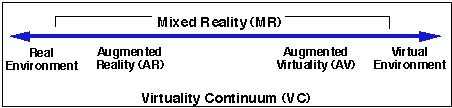
\includegraphics[width=0.6\textwidth]{../../Figures/milgram.jpeg} 
    \caption{Representation of the Reality-Virtuality Continuum by Milgram and Kishino \cite{milgram1994}.} 
    \label{fig:milgram} 
\end{figure}

In the context of schizophrenia, VR is often used to simulate intense experiences, such as auditory or visual hallucinations, representing psychosis. AR has been applied to embed simulated voices or visual cues into everyday settings, making the experience more relatable. MR, the focus of this thesis, seeks to integrate the strengths of both: allowing users to remain grounded in reality while experiencing interactive, layered symptoms, potentially leading to higher engagement and stronger emotional responses \cite{Krogmeier2024, Silva2017, Zare-Bidaki2022}.

\section{Immersive Simulations of Schizophrenia}
Immersive simulations have emerged as an important strategy to foster a better understanding of schizophrenia symptoms, as well as to address persistent stigma surrounding the disorder. Virtual Reality (VR) and Augmented Reality (AR) technologies are especially valuable, offering experiential learning environments where participants can “step into the shoes” of individuals experiencing hallucinations, delusions, or cognitive impairments \cite{Krogmeier2024}. These approaches have proven to be effective not only in increasing empathy and knowledge but also, in many cases, in reducing stigma among participants \cite{Krogmeier2024,Holopainen2023}.

\vspace{1em}

Recent developments have also emphasized the educational use of simulations targeted specifically at healthcare students and professionals, providing controlled, safe, and replicable experiences of psychotic symptoms to better prepare them for real-world clinical interactions \cite{Yoo2020,Lee2020}.

\subsection{Virtual Reality Applications}
Virtual Reality applications in the context of schizophrenia simulations typically seek to recreate sensory and cognitive disturbances through fully immersive experiences. These applications range from fully interactive environments developed with game engines like Unity to 360-degree videos played via head-mounted displays (HMDs) \cite{Yoo2020,Lee2020}. The use of VR allows users to experience symptoms of schizophrenia, such as auditory hallucinations, persecutory delusions, and visual distortions. Furthermore, VR interventions are now increasingly evaluated for their usability, realism, and educational effectiveness.

\subsubsection{Key Studies}

In the study by Zare-Bidaki et al., a Virtual Reality Simulation of Psychosis was designed based on interviews with real patients in remission. The experience placed users in a familiar, culturally grounded setting where they encountered persecutory auditory hallucinations (e.g., voices warning them not to open doors or mistrust others) and delusions of reference (e.g., the belief that a TV news anchor was speaking directly to them). This scenario-based simulation allowed students to embody a person experiencing a psychotic episode, moving through spaces such as a living room and kitchen while hearing distressing voices and observing realistic environmental triggers. The study found that such simulations were significantly more effective than standard clinical observation at reducing stigma and improving empathy and knowledge \cite{Zare-Bidaki2022}. Importantly, Zare-Bidaki et al.'s participants were medical students tasked with simulating the experience of a psychotic episode to enhance their clinical empathy and understanding.

\vspace{1em}

More recent work by Alieldin et al., although focusing on social isolation rather than schizophrenia per se, underscored the power of immersion, presence, and embodiment in fostering empathy. Their findings align with others in this field, emphasizing that VR-based empathy training is most impactful when the simulated symptoms are contextualized in relatable environments and paired with reflective debriefing \cite{Alieldin2024}.

Silverstein et al. and van Ommen et al. looked at how people with schizophrenia might see distorted images, such as unfamiliar faces, strange objects, or unreal environments \cite{Silverstein2021,Vanommen2019}. However, it is important to clarify that their works primarily explored the phenomenology of visual hallucinations in clinical schizophrenia, not through VR simulations, and not directly in educational interventions for students. Nonetheless, these insights become incredibly important, and were also heavily used for the design of the simulation created in this project, as they help to create a more realistic and relatable experience for users.

Specifically, in the schizophrenia simulation project by Domnick et al. \cite{Domnick2023}, users encountered visually altered settings such as pharmacies and grocery stores, where everyday things, like a bottle of pills, suddenly looked like a threatening object, like poison. Hallucinated figures appeared unexpectedly, and AI-generated voices with emotional modulation (anger or paranoia) created a tense auditory landscape. This simulation allowed users not only to hear internal voices but also to interact with them, fostering a dynamic understanding of psychosis symptoms.

\vspace{1em}

Furthermore, some tools are made specifically for training in medical and nursing education. Yoo et al. and Lee et al. developed VR training programs using 360-degree video and actors to recreate clinical situations \cite{Yoo2020, Lee2020}. The primary goal was to simulate encounters with patients exhibiting psychiatric symptoms in hospital settings. These tools largely rely on passive observation within pre-recorded 360° videos, meaning that while users can look around and witness events unfold, direct interaction with the environment is usually limited. Thus, while they offer vivid emotional realism, they often lack deep interactivity. These simulations included symptoms like hearing voices or patients behaving aggressively and were shown to be realistic and useful for learning.

\vspace{1em}

Tu summarize, these recent projects have shown how powerful immersive VR can be in medical education. Their VR tools recreated key symptoms of schizophrenia—like hearing distressing voices, feeling suspicious of others, feeling paranoid, or struggling to follow a clear train of thought, meaning cognitive disorganization. Unlike passive video experiences, these tools allowed medical students to actively move through the environment and experience the symptoms in real time. For instance, students might hear a voice whispering insults or warnings as they try to complete a task, or see unsettling figures appear suddenly in a grocery store. These immersive scenarios helped students not just observe the symptoms but feel what it is like to live with them, leading to stronger emotional engagement, better memory of the experience, and less stigma toward people with schizophrenia \cite{Kuhail2022,Domnick2023}. This aligns with findings from broader reviews of the field \cite{Lan2023,Bisso2020}, which emphasize that VR is especially effective when it combines multiple senses — like sight and sound — to show the complex reality of psychosis. When done thoughtfully, these simulations are not only safe and engaging, but also powerful tools for building empathy and improving mental health education.

\paragraph{Research Gaps}

While immersive technologies have become increasingly valuable for simulating schizophrenia symptoms, existing research remains heavily focused on VR. Among the broader XR spectrum, VR is by far the most studied and widely applied method, leaving AR and MR comparatively underexplored \cite{Kuhail2022}. As shown in Table~\ref{tab:studies}, there is a growing body of work exploring immersive technologies for empathy training. However, most studies focus on VR, with limited exploration of AR or MR. This supports the rationale for this thesis, which investigates the potential of MR-based simulations.

\vspace{1em}

For instance, a systematic review by Holopainen et al. examined 12 studies using VR-based interventions for schizophrenia, including cognitive behavioral therapy (CBT) or social skills training. These studies reported positive outcomes across a range of symptoms — such as hallucinations, paranoia, and cognitive difficulties — with minimal adverse effects. Notably, none of the reviewed interventions utilized AR or MR, further showing the gap in the literature \cite{Holopainen2023}.

\vspace{1em}

Similarly, Lan et al. reviewed a large number of articles and found that, while VR continues to show promise in these medical settings, there was no evidence of AR or MR being tested in medical trials for psychosis. Despite the many advantages these technologies could offer — particularly MR, which allows for immersive symptom simulation while keeping users aware that they remain in the real world \cite{Lan2023}.

This gap presents a good opportunity to explore MR as an alternative approach, especially for applications with the focus on empathy development. MR has the potential to provide emotionally engaging yet psychologically safer experiences than fully immersive VR. The following section highlights existing studies that have begun to explore AR and MR in schizophrenia education, and sets the foundation for the MR-based approach developed in this thesis.

\subsection{Augmented and Mixed Reality Applications}

Unlike fully immersive VR, AR and MR offer the unique ability to layer simulated symptoms onto the users real-world environment. This approach allows learners to remain grounded in familiar settings while still gaining insight into the experiences of people with schizophrenia. These technologies can make educational simulations more accessible, especially for those who may find full VR experiences overwhelming. The following studies illustrate how AR and MR have been used to simulate schizophrenia symptoms in interactive and educational ways.

\subsubsection{Key Studies}
\label{sec:keystudies}

An increasing number of studies are exploring the use of AR and MR in schizophrenia education. One early - and for this thesis very relevant - example is by Silva et al., who created a tool using AR to simulate psychotic symptoms. This system, developed with input from psychiatric professionals, was designed to help users — especially medical students — better understand schizophrenia and reduce stigma. The AR tool allowed users to interact with simulated symptoms in real time, providing a safe and controlled learning environment \cite{Silva2017}. Figure~\ref{fig:silva_ar_scene} illustrates how symptoms such as visual distortions were presented in the system. To test the system, 21 medical students used AR glasses (HMZ-T2, Sony glasses\footnote{\href{https://www.vrbrillen.net/sony-hmz-t2/}{Sony HMZ-T2 product page}}) to experience the simulation. Afterward, they filled out questionnaires about their attitudes toward schizophrenia, how realistic they found the experience, and whether their views had changed. Students gave high ratings for the audio quality and educational value of the simulation. Many said it helped them better understand what psychotic experiences might feel like. However, some users also reported problems, such as discomfort from the equipment and difficulty focusing in the environment \cite{Silva2017}. The simulations impact on empathy and stigma was measured using questionnaires before and after the experience. The results showed that students felt more empathy, expressed more concern for a fictional patient, and were more willing to help. However, there was also a small increase in stigma scores, showing that the results were complex. The study suggests that while AR can help increase empathy, future designs should focus on improving comfort and exploring long-term effects \cite{Silva2017}. It also recommends combining simulations with brief educational sessions on schizophrenia to deepen understanding \cite{Silva2017}. 


\begin{figure}[H]
  \centering
  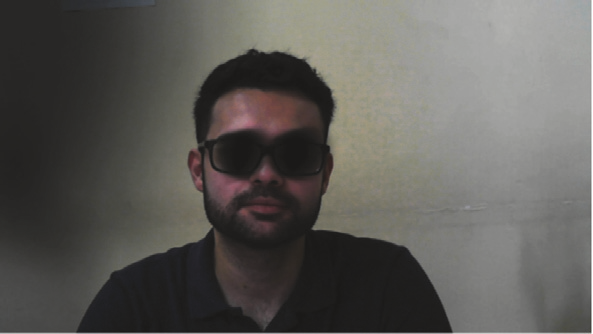
\includegraphics[width=0.4\textwidth]{../../Figures/silva_ar_scene.png}
  \caption{View from the AR simulation created by Silva et al., showing layered visual hallucinations designed to simulate psychotic experiences \cite{Silva2017}.}
  \label{fig:silva_ar_scene}
\end{figure}


\vspace{1em}

Another very relevant study by Skoy et al. created a simulation where users hear disturbing voices through headphones to better understand the kind of confusion and distraction that people with schizophrenia may deal with \cite{Skoy2016}. The simulation used Patricia Deegan's \emph{Hearing Distressing Voices} audio track — based on real personal experience with schizophrenia — and was paired with practical tasks. Students completed these while listening to disturbing voices through headphones, mimicking real-life challenges. The audio track itself includes a range of disturbing content. Some voices whisper critical comments like \emph{"You're stupid"} or \emph{"Don't trust them."} Others issue confusing commands such as \emph{"Pick it up!"} or \emph{"Go to the corner!"} Occasionally, the voices escalate into more aggressive or paranoid content, saying things like \emph{"They’re watching you"} or \emph{"Everyone knows what you did."} These auditory hallucinations mimic how real-life psychotic symptoms can shift unpredictably from confusing to threatening. The combination of conflicting, emotional, and nonsensical input creates a sense of mental overload and disorientation. After the simulation, students took part in a debriefing and completed reflective writing. Results showed a significant increase in empathy scores \cite{Skoy2016}.

\vspace{1em}

Chaffin et al. presented a more focused simulation using the same \emph{Hearing Distressing Voices} track. In this intervention, students were asked to perform everyday tasks—such as grocery shopping or engaging in conversation—while listening to the same pre-recorded track of intrusive, distressing voices. This approach highlighted again how such symptoms disrupt cognition, focus, and interpersonal interaction. Students reported transformative experiences, reflecting on the difficulty of completing simple tasks and expressing increased patience and understanding toward patients \cite{Chaffin2013}.

\vspace{1em}

A more recent project by Krogmeier et al. introduced \textit{Live-It}, an augmented reality  simulation designed to help people better understand what it is like to live with schizophrenia. The system used the passthrough feature of the Meta Quest 3 headset, which allows users to see their real surroundings while digital hallucinations and delusions are layered on top. Unlike fully immersive VR, \textit{Live-It} placed these experiences in everyday environments, like a living room, making the symptoms feel more realistic and relatable \cite{Krogmeier2024}. One example was a scenario involving a television. As users looked at the screen, they saw a normal news broadcast gradually change. The news anchor appeared to speak directly to them, hinting that they were being watched or targeted. This scene illustrated a common type of delusion known as delusions of reference, where people believe that neutral events, like a TV-show, are specifically about them.  A visual from this moment in the simulation is shown in Figure~\ref{fig:liveit_tv}, where the user, seated in a familiar room, sees the news anchor addressing them by name. Besides this, users might also hear voices commenting on their actions or giving conflicting instructions, mimicking the experience of auditory hallucinations. Other symptoms were presented throughout the simulation. Participants reported hearing voices that ranged in tone—some critical or paranoid, others calm or supportive—reflecting the emotional variety of real-life auditory hallucinations. Visually, objects could shift or appear distorted, and shadowy figures might be seen out of the corner of the eye. 

\begin{figure}[H]
  \centering
  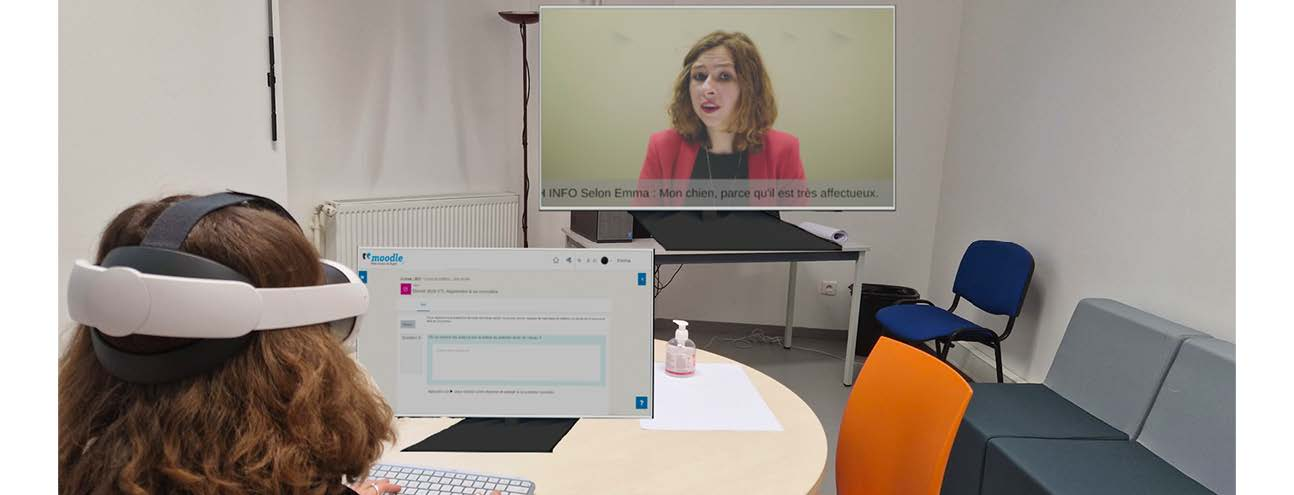
\includegraphics[width=0.6\textwidth]{../../Figures/live-it.jpeg}
  \caption{Scene from the \textit{Live-It} AR simulation showing a delusion of reference involving a news broadcast \cite{Krogmeier2024}.}
  \label{fig:liveit_tv}
\end{figure}

The content was based on interviews with individuals who live with schizophrenia and was reviewed by mental health professionals to ensure it was both accurate and respectful. Participants in the study, mainly students and mental health professionals, said the simulation was powerful, emotional, and helped them better understand what living with schizophrenia might feel like. Importantly, the experience ended with a hopeful message, reminding users that people with schizophrenia can still live fulfilling lives. Overall, \textit{Live-It} showed how AR can be a valuable tool in mental health education. By embedding symptoms into real-life situations, like watching TV, it made the experience feel authentic without being overwhelming, helping users connect theory with lived experience \cite{Krogmeier2024}.


\paragraph{Technical Advantages}

AR/MR simulations place symptoms in real-world settings, which can reduce user discomfort and improve relatability. These simulations tend to be less intense than full VR, making them more accessible to first-time users or those unfamiliar with immersive technology. One useful feature is passthrough, a technology that allows users to see their actual surroundings through cameras on the headset while digital content is overlaid on top. This helps users stay oriented and grounded in the real world while still experiencing simulated symptoms, which may enhance engagement while minimizing sensory overload. Features like passthrough may help enhancing empathy without overwhelming users \cite{Krogmeier2024, Silva2017, Lan2023}.

\section{Empathy in Healthcare Education}

Empathy is one of the most important skills in healthcare. It helps doctors, nurses, and other professionals connect with their patients in a real and meaningful way. Before we look at how empathy is taught or tested, it is helpful to understand what it actually means and why it matters so much in medical and nursing education.

\subsection{Definition of Empathy}
Empathy is a key part of good communication and care in healthcare. Many studies have shown that when healthcare professionals show empathy, patients are more satisfied, more likely to follow treatment plans, and often have better mental health outcomes \cite{Cunico2012, Olson1995, Ozcan2018}. In medical and nursing education, empathy is no longer seen as just a "soft skill." It is now treated as something important that can be taught and developed. Teaching empathy helps improve the way future professionals connect with patients and provide care \cite{Cunico2012}.

\vspace{1em}

Empathy is usually described as having two main parts: \textit{cognitive empathy} and \textit{affective empathy}. Cognitive empathy is the ability to understand what someone else is thinking or feeling. Affective empathy means actually feeling or emotionally connecting with what the other person is going through \cite{Ventura2020, Martingano2021}. In healthcare, both types are important. Understanding a patient's perspective (cognitive empathy) helps with communication and decision-making, while emotional connection (affective empathy) helps build trust and stronger relationships \cite{Cunico2012, Ozcan2018}.  Understanding this and training empathy helps doctors and nurses better understand their patients and respond in helpful and compassionate ways \cite{Ozcan2018, Olson1995}. However, research has shown that empathy can decrease during medical training. This might be because students are under pressure, focusing more on technical knowledge, or feeling emotionally drained \cite{Mattsson2024, Ozcan2018}. This decline in empathy can lead to negative outcomes for both patients and healthcare professionals. Patients may feel misunderstood or neglected, while healthcare providers may experience burnout and job dissatisfaction \cite{Mattsson2024, Cunico2012}. Therefore, it is crucial to find effective ways to teach and maintain empathy in medical education.

\paragraph{Measuring Empathy}
Various instruments are used to measure these dimensions of empathy, including the Jefferson Scale of Empathy (JSE), which is being widely applied in medical education \cite{Alieldin2024}. This tool allows researchers to assess changes in empathy following interventions and distinguish between shifts in emotional versus cognitive components, which is also what I want to achieve in this thesis. In the context of this thesis, the JSE will be used to measure the impact of the MR simulation on medical students' empathy levels. The JSE is a validated instrument that has been widely used in medical education research and has demonstrated reliability and validity in assessing empathy in healthcare professionals \cite{Hojat2002}. 

\subsection{Immersive Technologies and Empathy}

Empathy training in healthcare education has traditionally relied on methods like role-playing, patient interviews, and reflective writing \cite{Batt-Rawden2013}. However, these approaches often struggle to create the deep emotional engagement needed to truly understand the experiences of patients with mental health conditions like schizophrenia \cite{Hsia2022, Formosa2018}. Immersive technologies like VR and MR offer new ways to enhance empathy by allowing users to experience symptoms from a first-person perspective \cite{Krogmeier2024, Silva2017}.

\subsubsection{Empathy Increase through Virtual Reality}

Virtual Reality (VR) has often been called the "ultimate empathy machine" because it can create powerful first-person experiences in fully immersive environments \cite{Milk2015}. Several studies support this idea, showing that VR can have a strong emotional effect on users.

VR is especially useful when it comes to helping people understand the experiences of stigmatized groups, which individuals with schizophrenia also belong to \cite{Formosa2018, Marques2022, Mattsson2024}. By placing users in situations that reflect what it might be like to live with psychosis, these simulations aim to increase empathy and reduce negative attitudes. For example, a study by Hsia et al. showed that pharmacy students who experienced auditory hallucinations in VR also became more empathetic and less stigmatizing toward people with schizophrenia \cite{Hsia2022}. One crucial reason for this was that the students also heard from a guest speaker diagnosed with schizophrenia after they have experienced the simulation. This combined approach helps address one of the main concerns with simulations — that they can unintentionally increase social distance or reinforce stereotypes if not supported by real-life context. Including authentic human interaction can make the experience more meaningful and well-rounded. In this thesis we will also include a debriefing session after the simulation, where students can reflect on their experiences and discuss them with peers and instructors. This is important for helping students process what they have learned and apply it to real-life situations \cite{Hsia2022}.

\vspace{1em}

A recent mixed-methods study by Alieldin et al. tested the use of immersive virtual reality to improve empathy among first-year medical students \cite{Alieldin2024}. The intervention involved a VR simulation which placed students in the perspective of “Frank,” a socially isolated 72-year-old man. Students experienced the story from a first-person viewpoint and encountered situations related to grief, health decline, loneliness, and difficulties with daily life. Empathy levels were measured before and after the training using the Jefferson Scale of Empathy (JSE). Students showed a statistically significant increase in empathy scores. In post-session interviews, participants described the simulation as powerful, emotional, and immersive. These emotional responses were complemented by cognitive empathy, with students explaining how they better understood the struggles older adults face, especially with healthcare access and family relationships. The study also conducted follow-up interviews six months later. Students still remembered the experience vividly and reported applying what they had learned in patient interactions and standardized clinical scenarios. Importantly, the debriefing after the simulation was seen as a crucial component — helping students reflect, connect the experience to real-life practice, and deepen their learning. These results show how virtual reality can support both short-term empathy development and also have an effect on the longer-term, which supports the argument for immersive simulations in healthcare education \cite{Alieldin2024}.

\vspace{1em}

Formosa et al. tested a custom-built VR simulation designed to show what it feels like to experience positive symptoms of psychosis, such as auditory and visual hallucinations and paranoid thoughts \cite{Formosa2018}. Fifty participants — including students and people from the general public — completed a short immersive scenario inside a virtual house, where they heard disturbing voices, saw shadowy figures, and experienced delusions based on a fictional character’s background story.The researchers measured empathy, knowledge, and attitudes before and after the simulation. Results showed a significant increase in all three areas. Participants scored higher in understanding schizophrenia symptoms, felt more empathy, and reported more positive attitudes afterward. Interestingly, the simulation included no formal teaching — just the immersive experience itself. This supports the idea that experiencing symptoms directly can be a powerful learning tool. The study also looked at how much participants "believed" the simulation. People who felt the experience was realistic and useful showed the biggest increase in empathy. This shows that emotional connection and meaningful design are key when using VR for education. 

\vspace{1em}

While VR has shown strong results in building empathy, it is not the only option. MR is becoming more popular because it blends digital effects with the real world, making the experience feel more grounded and less overwhelming. The next section will take a look at how MR is being used to simulate mental health symptoms in a way that feels real but also safe and manageable for students.

\subsubsection{Empathy Increase through Mixed Reality}

MR is gaining attention as a promising alternative to VR in empathy-focused education, particularly in mental health contexts. Unlike VR, MR allows users to remain partially connected to their physical surroundings while engaging with digitally simulated symptoms. This hybrid approach combines the immersive power of VR with the real-world anchoring of AR, helping to reduce sensory overload and making experiences more relatable and less overwhelming \cite{Zare-Bidaki2022}.

Studies by Silva et al. and Krogmeier et al., which were already discussed in detail in section~\ref{sec:keystudies} demonstrate the effectiveness of MR in increasing empathy and understanding toward individuals with schizophrenia. In both cases, simulations placed users in familiar environments while layering auditory and visual hallucinations over the reality. Participants reported strong emotional engagement and a clearer understanding of what it might be like to experience psychosis \cite{Silva2017, Krogmeier2024}. 

\vspace{1em}

Together, these insights reinforce the central aim of this thesis: to evaluate MR as a balanced and effective tool for simulating psychotic experiences in medical education. By allowing users to engage empathetically with symptoms while staying cognitively oriented, MR may better support both affective and cognitive empathy development. Its ability to blend emotional immersion with realism makes it especially well-suited for sensitive topics like schizophrenia, where responsible storytelling and psychological safety are essential.

\subsection{Limitations in Empathy Training}
\label{sec:limitationsempathytraining}

Martingano et al. reviewed 43 studies and found that while VR often enhances affective empathy, its effect on cognitive empathy is less consistent \cite{Martingano2021}. They argue that immersive experiences might reduce the user's need to mentally simulate another's perspective, as the simulation does that work for them. Without reflection or guided discussion, users may have strong emotional reactions but fail to develop deeper understanding. Similarly, Mattsson et al. found that while VR can increase empathy, it does not necessarily lead to long-term changes in attitudes or behaviors \cite{Mattsson2024}. They suggest that without structured debriefing or reflection, the emotional impact of VR experiences may fade quickly, leaving users with little more than a fleeting emotional response.

\vspace{1em}

Moreover,  a meta-analysis by Ventura et al. reviewed existing studies to see whether virtual reality can help increase empathy or perspective-taking \cite{Ventura2020}. The researchers analyzed data from seven studies and nine different participant groups. Overall, they found that VR had a moderate, statistically significant effect on perspective-taking — meaning users became better at imagining things from another persoNs point of view. However, the impact on empathy itself was smaller and not statistically significant. This suggests that VR may be more effective at helping people understand others (\textit{cognitive empathy}) than at creating deep emotional connection (\textit{affective empathy}). The authors also noted that how the VR is designed matters: experiences that include a strong sense of presence - like "being there" - or embodiment - like “being someone else” - may be more effective. 

\vspace{1em}

Similarly, Rueda and Lara caution against relying on emotional responses alone. They call for "reason-guided empathy," which integrates critical thinking and ethical reflection into simulation-based learning \cite{Rueda2020}. Without this, empathy may be short-lived or biased. The findings also show that more expensive or immersive setups do not necessarily yield better outcomes. Thoughtful design and context are incredibly important. Many VR simulations rely heavily on dramatic intensity, which can restrict the ability of the user to reflect or exercise perspective-taking — the cognitive process of imagining the world from another persons viewpoint, which is essential for developing empathy and reducing bias \cite{Mattsson2024}. This limitation further supports the use of MR paired with preparation and debriefing, as adopted in this thesis.

Additionally, Ozcan et al. tracked empathy development in nursing students over four years. While communication skills improved, emotional empathy declined—likely due to burnout or emotional distancing \cite{Ozcan2018}. This underlines the importance of designing empathy training that includes emotional support and reflection and a simulation which could be used repeatedly to be refreshed over the years. The MR simulation in this thesis builds on that principle.

\vspace{1em}

Finally, as mentioned repeatedly, ethical concerns remain. VR simulations can unintentionally reinforce negative stereotypes if not carefully framed. Being incredibly affected by something, without deeper context, may lead to bias or stigma \cite{Rueda2020}. MR used in the real world, along with structured pre- and post-simulation activities, is intended to reduce this risk. The approach in this thesis prioritizes both emotional resonance and cognitive clarity to improve thoughtful empathy in clinical learners.


\section{Simulation Design Considerations}

Immersive simulations offer powerful opportunities to increase empathy in medical education, particularly for conditions like schizophrenia. However, designing effective simulations requires careful attention to realism, emotional impact, and usability. This means paying close attention to how the experience looks, sounds, and feels, not just for emotional impact, but also for how easy it is to use and understand. The next section looks at how these design choices can influence empathy and what researchers have learned from past simulations.

\subsection{Empathy and Usability}

Marques et al. compared a VR simulation of psychosis with a standard 2D video and found that the VR group experienced greater gains in cognitive empathy and held more positive attitudes toward individuals with schizophrenia. However, the study also noted several limitations: it lacked a control group and did not measure perceived immersion — a key factor in empathy development. Some participants also struggled with unfamiliarity with the technology \cite{Marques2022}. Similarly, Zare-Bidaki et al. found that VR simulations of psychosis led to higher empathy and stigma reduction compared to traditional patient visits. However, they emphasized that simulations should supplement and not replace direct human interactions. Authentic contact provides depth, variability, and personal meaning, which simulations alone cannot replicate \cite{Zare-Bidaki2022, Hsia2022}.

\vspace{1em}

Both studies emphasize that simulations must balance engagement and emotional intensity without overwhelming participants. Overly dramatic portrayals of symptoms — such as frightening hallucinations or paranoia — can trigger distress, increase social distance, or reinforce harmful stereotypes if not properly contextualized \cite{Ando2011, Chaffin2013, Zare-Bidaki2022}. To reduce this risk, Zare-Bidaki et al. recommend using calm, familiar environments and grounding simulations in lived experience. They also suggest that AR or MR, which preserve awareness of the real world, may help avoid overstimulation while still enabling emotional immersion \cite{Zare-Bidaki2022}. This aligns with the approach taken in this thesis, which uses MR to simulate symptoms in relatable real-world contexts. The use of passthrough features allows participants to remain anchored while interacting with hallucination overlays, aiming to increase empathy without sensory overload.

\vspace{1em}

While immersive simulations have a lot of potential to improve empathy, they also come with some serious responsibilities. If not designed carefully, they can actually backfire—causing confusion, reinforcing stereotypes, or overwhelming students. In the next part, the ethical questions that come up when using these tools in mental health education are explored, and why reflection and thoughtful storytelling are just as important as the technology itself.

\subsection{Ethical Challenges}
\label{sec:ethicalchallenges}

While immersive simulations hold great promise for enhancing empathy, they also raise important ethical and psychological concerns—particularly in the context of mental health education as seen in the previous sections. Many studies suggest that emotional impact alone does not guarantee positive attitudinal change and may, in some cases, increase discomfort or misunderstanding \cite{Ando2011}.

These findings highlight the critical importance of proper preparation and debriefing. Without guided reflection, users may interpret psychotic symptoms in simplistic or be afraid of them, reinforcing stereotypes about schizophrenia. Ando et al. and Rueda and Lara both advocate for what they call a \textit{reason-guided empathy}, a model in which emotional engagement is supported by ethical reflection and cognitive understanding. This approach encourages users not only to feel compassion but also to think critically about the lived experience of mental illness \cite{Ando2011, Rueda2020}. 

\vspace{1em}

Another important ethical issue has to do with how the simulation is designed. Using very realistic effects, like intense visuals, surround sound, and dramatic symptoms, can make the experience feel more lifelike. But for some users, especially those not used to immersive technology, this can be overwhelming. Also, trying to show a typical psychotic episode can be problematic, since symptoms vary a lot from person to person. This could lead to a simplified or even misleading picture of what schizophrenia is really like \cite{Zare-Bidaki2022}.

It is also essential to think about how the story behind the symptoms is presented. If the simulation focuses only on fear or confusion without any background or explanation, it might unintentionally make people with schizophrenia seem dangerous or unstable. Rueda and Lara warn that mental health simulations need to be told in a responsible way—showing the human side of the experience, not just the symptoms \cite{Rueda2020}.

\vspace{1em}

In conclusion, when used alongside proper educational materials and opportunities to reflect on the experience, MR can help build deeper, more respectful empathy. 

\section{Overview of Relevant Studies}
To consolidate the findings discussed in this chapter, Table~\ref{tab:studies} presents an overview of the key studies referenced. It summarizes the study designs, technologies used, symptom types, target audiences, and their effects on empathy and stigma. This table helps highlight the diversity of approaches and the gaps in existing research, particularly with regard to MR-based studies, which this thesis aims to address.

\newcolumntype{P}[1]{>{\raggedright\arraybackslash}p{#1}}
\begin{landscape}
    \footnotesize	
    \begin{longtable}{|P{2.8cm}|P{0.6cm}|P{1.8cm}|P{1.2cm}|P{1.2cm}|P{2cm}|P{1.2cm}|P{1.2cm}|P{1.2cm}|P{3cm}|}
    \caption{Overview of studies used for this thesis} \label{tab:studies} \\
    \hline
    \textbf{Title} & \textbf{Year} & \textbf{Study Design} & \textbf{Tools Used} & \textbf{Target Group} & \textbf{Symptom Experience} & \textbf{Empathy or Stigma} & \textbf{Cognitive Empathy Increased} & \textbf{Affective Empathy Increased} & \textbf{Main Results} \\
    \hline
    \endfirsthead
    \hline
    \textbf{Title} & \textbf{Year} & \textbf{Study Design} & \textbf{Tools Used} & \textbf{Target Group} & \textbf{Symptom Experience} & \textbf{Empathy or Stigma} & \textbf{Cognitive Empathy Increased} & \textbf{Affective Empathy Increased} & \textbf{Main Results} \\
    \hline
    \endhead
    Impact of a Virtual Reality-Based Simulation on Empathy and Attitudes Toward Schizophrenia & 2022 & Quasi-experimental & VR & Health students & Simulated psychotic symptoms & Both & Yes & Possibly & VR more effective than 2D video in enhancing empathy and reducing stigma \\
    \hline
    Nursing Students' Experiences of Empathy in a Virtual Reality Simulation Game & 2024 & Descriptive qualitative & VR & Nursing students & Virtual patient care & Empathy & Yes & Yes & VR helped students experience and express empathy effectively \\
    \hline
    Virtual Reality as a Medium to Elicit Empathy: A Meta-Analysis & 2020 & Meta-analysis & VR & Various populations & Multiple contexts & Empathy & Yes & Unclear & Perspective-taking improved; general empathy results were mixed \\
    \hline
    Testing the efficacy of a virtual reality based simulation in enhancing users' knowledge, attitudes and empathy relating to psychosis & 2018 & Experimental pre-post & VR & General public, psychology students & Simulated psychotic symptoms & Both & Yes & Yes & VR simulation significantly increased empathy, knowledge, and improved attitudes \\
    \hline
    Virtual Reality and Empathy Enhancement: Ethical Aspects & 2020 & Theoretical Review & VR & General & Not specific (broad scenarios) & Empathy & Possibly & Possibly & Explores philosophical and ethical aspects; emphasizes reason-guided empathy over immersive emotion \\
    \hline
    Effectiveness of immersive virtual reality in teaching empathy to medical students & 2024 & Mixed methods (pre-post + interviews) & VR & Medical students & Social isolation in older adults & Empathy & Yes & Yes & Empathy significantly increased post-training; immersion and embodiment were key factors \\
    \hline
    VR Improves Emotional but Not Cognitive Empathy: A Meta-Analysis & 2021 & Meta-analysis & VR & General population & Various contexts & Empathy & No & Yes & VR improved emotional empathy but not cognitive empathy; not more effective than less technical methods \\
    \hline
    The Virtual Doppelganger: Effects of a Virtual Reality Simulator on Perceptions of Schizophrenia & 2010 & Between-subjects experiment & VR & General public & Schizophrenia symptoms & Both & Yes & Yes & Empathy + VR condition most effective; VR-only increased desire of social distance \\
    \hline
    Immersive VR Applications in Schizophrenia Spectrum Therapy: A Systematic Review & 2020 & Systematic review & VR & Patients with schizophrenia  & Delusions, hallucinations, cognitive/social issues & Empathy (implied), Therapy & Not directly measured & Not directly measured & VR showed promising results for therapy; safe and well tolerated \\
    \hline
    Efficacy of Immersive XR Interventions on Symptoms of Schizophrenia Spectrum Disorders & 2023 & Systematic review & XR (VR) & Patients with schizophrenia & Various psychotic symptoms & Empathy, Therapy & Not focus & Not focus & VR effective across symptom domains; no AR studies found \\
    \hline
    Representing Mental Disorders with Virtual Reality: Goliath & 2023 & Case study analysis & VR & General public & Narrative VR of schizophrenia & Empathy & Yes & Yes & Focused on ethical, artistic VR design for empathy through embodiment \\
    \hline
    Immersive Simulation of Schizophrenia & 2023 & Development and evaluation project & VR & General public / students & Visual and auditory hallucinations & Stigma & Possibly & Possibly & VR simulation aimed to reduce stigma; immersive experience showed promise for education \\
    \hline
    Learning by Doing: Educational VR for Care of Schizophrenic Patients & 2020 & Design and usability study & VR  & Nursing students & Various schizophrenia symptoms & Empathy & Possibly & Yes & Participants reported increased empathy and engagement; useful educational platform \\
    \hline
    Evaluating VR Simulation of Psychosis on Stigma, Empathy, and Knowledge & 2022 & Controlled experimental & VR & Medical students & Psychotic symptoms & Both & Yes & Yes & VR significantly more effective than ward visits at increasing empathy and reducing stigma \\
    \hline
    Usability of Mental Illness Simulation via Immersive VR & 2020 & Mixed methods usability study & VR & Nursing students & Schizophrenia symptoms & Empathy & Possibly & Yes & Students found simulation realistic and engaging; suggested for broader use in nursing education \\
    \hline

    Reducing the Schizophrenia Stigma: A New Approach Based on Augmented Reality & 2017 & Quasi-experimental & AR & Medical students & Psychotic symptoms simulation & Stigma & Not measured & Not measured & AR experience reduced stigma and improved understanding of schizophrenic symptoms \\
    \hline
    Leveraging AR for Understanding Schizophrenia & 2024 & Thematic evaluation (qualitative) & AR & Healthcare students, experts & Hallucinations, delusions, disorganized behavior & Stigma & Possibly & Possibly & Participants better understood schizophrenia; highlighted as an educational tool \\
    \hline
    Empathic Mixed Reality: Sharing What You Feel and Interacting with What You See & 2017 & Experimental (early studies) & MR (AR + VR) & General users (not specified) & Emotion sharing, collaboration & Empathy & Possibly & Yes & MR enabled physiological and emotional data sharing; promising for collaborative empathy \\
    \hline
    The Simulation of Hallucinations to Reduce the Stigma of Schizophrenia: A Systematic Review & 2011 & Systematic review & Audio Simulation & Mixed (students, general public) & Hallucination simulation & Stigma & No & Yes & Increased empathy, but also social distance; ethical considerations advised \\
    \hline
    Impact of an Auditory Hallucination Simulation Coupled with a Speaker Diagnosed with Schizophrenia & 2022 & Pre-post with speaker intervention & Audio simulation & Pharmacy students & Auditory hallucinations & Stigma & Not focus & Not focus & Stigma reduced significantly, especially in attitudes and disclosure openness \\
    \hline
    Creating Empathy Through Use of a Hearing Voices Simulation & 2013 & Mixed methods (pre-post and reflection) & Audio simulation & Psychiatric nursing students & Auditory hallucinations & Empathy & Not measured & Yes & Empathy significantly increased; students reported transformation in attitude and care approach \\
    \hline

    Use of an Auditory Hallucination Simulation to Increase Student Pharmacist Empathy & 2016 & Pre-post experimental & Audio simulation & Pharmacy students & Auditory hallucinations & Empathy & Not measured & Yes & Empathy increased; students reported distraction and frustration during task \\
    \hline
    Developing empathy in nursing students: a cohort longitudinal study & 2012 & Cohort longitudinal & Traditional education methods & Nursing students & General emotional and communication contexts & Empathy & Yes & Yes & Empathy improved significantly in women through targeted training; results less clear for men \\
    \hline
    Improving Empathy in Nursing Students: A Comparative Longitudinal Study of Two Curricula & 2018 & Comparative longitudinal & Traditional vs. integrated curriculum & Nursing students & General emotional and clinical context & Empathy & Yes & Decreased over time & Integrated curriculum more effective; empathic skills improved but tendency declined \\
    \hline
    Relationships Between Nurse\textendash Expressed Empathy, Patient\textendash Perceived Empathy and Patient Distress & 1995 & Correlational study & Standard clinical practice & Nurses and patients & Real-life distress in hospital settings & Empathy & Not applicable & Not applicable & Nurse-expressed empathy positively correlated with perceived empathy; reduced patient distress \\
    \hline
    Out of Touch with Reality? Social Perception in First-Episode Schizophrenia & 2013 & fMRI observational study & None & Schizophrenia patients & Tactile and social perception stimuli & Empathy & Impaired (linked to self-other confusion) & Not measured & Impaired neural mechanisms for social touch perception; linked to empathy deficits \\
    \hline
    Visual Hallucinations in Psychosis & 2019 & Clinical observational study & None & Psychosis patients & Visual hallucinations (VH) & Empathy (implied) & Not measured & Not measured & VH are diverse and vivid; associated with reduced insight and fear; linked to stigma and distress \\
    \hline
    Visual Distortions and Hallucinations in Schizophrenia: An Update & 2021 & Literature review & None & Schizophrenia patients & Visual hallucinations and distortions & Empathy (conceptual) & Not directly assessed & Not directly assessed & Explores mechanisms and clinical impact of visual symptoms; calls for targeted interventions \\
    \hline
\end{longtable}
\end{landscape}
